\documentclass{report}
\usepackage{hyperref} % For hyperlinks in the document
\usepackage{longtable} % For tables that span multiple pages
\usepackage{graphicx} % For including graphics
% chktex-file 44
% chktex-file 38
% chktex-file 8

\title{Project 4: Home Security System Proposal}
\author{Logan williamson, Casey Curran, Lily Danforth, Tre Thacker, \\ Julissa Ramirez, Michael Bergman \\ Team 7}
\date{\today}

\begin{document}

\maketitle

\tableofcontents
\newpage

\chapter{Description of Project}
\section{Project Idea}
This proposal is for a home security system that is a hardware and software solution.
Our company will offer installation services for the system, which is a base station and various POE IP cameras.
The storage for the system will be through AWS and there will be a web interface to access the recorded feeds.
The monetization will be through a hardware and install fee, and a monthly subscription fee for the AWS storage and web interface.

The hardware will be based of a Raspberry Pie 5, with a Corral Accelerator, and a POE switch.
It will all be contained within a custom case that will be mounted to the wall.
The cameras will be POE IP cameras that will be connected to the switch and powered by it.
The customer will be able to pick various numbers and variations of indoor and outdoor cameras.

The Pie will be running the default version of Raspbian.
The open source software Frigate will be used to manage the cameras, feeds, recordings, and detection.
The storage will be through AWS S3 mounted locally using Rclone.
Frigate will handle the web interface, but there will be a tunnel to the AWS instance so the customer can access the recordings on the web.

The install service will be done by in house contractors.
They will visit the customer's home, advise them on number of cameras and camera placement.
They will then install the hardware, connect it to the internet, and show the customer how to use the system.


\chapter{Likely Marketing Efforts}
\section{Target Audience}
Our primary target market is homeowners, small business owners, and property managers who seek an affordable, high-tech security solution. 
Families who wish to enhance safety and businesses that require high-level surveillance will all be catered to by this system. 
By selling to homeowners, businesses, and security-conscious consumers, our AI-powered security system fills a sizable niche in the market. 
\section{Cost Expectations}
Testing Testing Testing

\chapter{Technical Details / Technical Research}
A three-tier surveillance security system package specifically designed for family homes. 
The packages offer different levels of security, from essential home monitoring to advanced surveillance with AI-based detection. 
Each package includes necessary hardware, software, and storage solutions for easy installation and use. 
The Coral USB Accelerator is included in all packages to enhance AI-based motion detection and object recognition. 
Real pricing for PoE switches has also been incorporated. 
Camera specifications have been adjusted so that the first tier supports either indoor or outdoor use, and the second tier includes both indoor and outdoor cameras.

Tier 1: Essential Home Package
The Essential Home Package is designed for families looking for an entry-level yet effective surveillance system. 
This package includes two cameras that can be used either indoors or outdoors, providing flexibility for home security.
Components:
\begin{itemize}
    \item 2 Indoor/Outdoor PoE Cameras (Reolink 5MP, 2560$\times$1920 resolution, 30 fps) - \$70 each
    \item 1 Raspberry Pi 5 (4GB RAM) pre-installed with surveillance software - \$60
    \item 1 Coral USB Accelerator for AI-powered motion detection - \$25.99
    \item 1 PoE Switch (4-port TP-Link TL-SF1005P) - \$40
\end{itemize}
\textbf{Features:}
\begin{itemize}
    \item Local storage on Raspberry Pi 5 (up to 128GB via microSD)
    \item Mobile app access for live viewing
    \item AI-based motion detection and object recognition using Coral USB Accelerator
\end{itemize}
\textbf{Estimated Total Cost:} \$266

\textbf{Tier 2: Smart Home Package}

This package offers additional security coverage and smart features for homeowners seeking more control over their surveillance system. It includes a combination of indoor and outdoor cameras, ensuring comprehensive security coverage.

\textbf{Components:}
\begin{itemize}
    \item 2 Indoor PoE Cameras + 2 Outdoor PoE Cameras (Reolink 5MP, 2560$\times$1920 resolution, 30 fps) - \$70 each
    \item 1 Raspberry Pi 5 (4GB RAM) pre-installed with surveillance software - \$60
    \item 1 Coral USB Accelerator for AI-powered motion detection - \$25.99
    \item 1 PoE Switch (8-port NETGEAR GS308PP) - \$100
\end{itemize}
\textbf{Features:}
\begin{itemize}
    \item Local storage on Raspberry Pi 5 (up to 256GB via external SSD)
    \item Mobile app access for live viewing and playback
    \item AI-based human and vehicle recognition for smarter motion detection
\end{itemize}
\textbf{Estimated Total Cost:} \$506

\textbf{Tier 3: Advanced Family Package}

The Advanced Family Package is ideal for families wanting full security coverage with AI-based surveillance features and cloud storage options. This package includes six cameras that can be used in any combination of indoor or outdoor settings.

\textbf{Components:}
\begin{itemize}
    \item 6 Indoor/Outdoor PoE Cameras (Reolink 5MP, 2560$\times$1920 resolution, 30 fps) - \$70 each
    \item 1 Raspberry Pi 5 (8GB RAM) pre-installed with surveillance software - \$80
    \item 1 Coral USB Accelerator for AI-powered motion detection - \$25.99
    \item 1 PoE Switch (16-port TP-Link TL-SG1016PE) - \$180
\end{itemize}
\textbf{Features:}
\begin{itemize}
    \item Local storage on Raspberry Pi 5 (up to 512GB via external SSD)
    \item Mobile app access for live viewing, playback, and two-way audio
    \item AI-powered motion detection and object recognition using Coral USB Accelerator
    \item Optional cloud storage integration with AWS
\end{itemize}
\textbf{Estimated Total Cost:} \$826

\section{Staffing and Salaries}

\textbf{Department Director:} \$180k/yr

\textbf{Software Team:}
\begin{itemize}
    \item \textbf{Business Analyst/Scrum Master:} \$120k/yr
    \item \textbf{Software Dev Lead}
    \begin{itemize}
        \item \textbf{Team 1:}
        \begin{itemize}
            \item \textbf{Senior Dev:} \$120k/yr
            \item \textbf{Junior Dev:} \$80k/yr
            \item \textbf{Junior Dev:} \$80k/yr
        \end{itemize}
        \item \textbf{Team 2:}
        \begin{itemize}
            \item \textbf{Senior Dev:} \$120k/yr
            \item \textbf{Junior Dev:} \$80k/yr
            \item \textbf{Junior Dev:} \$80k/yr
        \end{itemize}
    \end{itemize}
\end{itemize}

\textbf{Systems Team:}
\begin{itemize}
    \item \textbf{Systems Administrator:} \$80k/yr
    \item \textbf{Network and Security Lead:} \$120k/yr
    \begin{itemize}
        \item \textbf{Network and Security Specialist:} \$100k/yr
    \end{itemize}
    \item \textbf{Helpdesk Lead/External Liaison:} \$50k/yr
    \begin{itemize}
        \item \textbf{Helpdesk Specialist:} \$30k/yr
        \item \textbf{Helpdesk Specialist:} \$30k/yr
        \item \textbf{Helpdesk Specialist:} \$30k/yr
    \end{itemize}
\end{itemize}



\chapter{Defined Goals / MVP}
The end product is a home security system and hardware solution that we offer install services for. 
The package to the user will be home base station that has a POE switch, and varying IP cameras to connect to it. 
The storage for the system will be through AWS and the there will be a web interface to access the recorded feeds. 
The monetization is through a hardware and install fee, and a monthly subscription fee for the AWS storage and web interface. 

\chapter{Testing to be Performed}
\begin{longtable}{|p{3cm}|p{3cm}|p{3cm}|p{3cm}|}
\hline
\textbf{Requirements} & \textbf{Test Case} & \textbf{Test Result} & \textbf{Defect/Error}\\
\hline
\textbf{Hardware Setup} &  &  &  \\
\hline
Gather all required components & Verify all components are present &  &  \\
\hline
Insert the microSD card into the Raspberry Pi & Verify microSD card is inserted &  &  \\
\hline
Connect the Raspberry Pi to a monitor, keyboard, and mouse & Verify connections &  &  \\
\hline
Power on the Raspberry Pi & Complete initial setup wizard &  &  \\
\hline
\textbf{Raspberry Pi OS Configuration} &  &  &  \\
\hline
Download Raspberry Pi Imager & Verify download &  &  \\
\hline
Flash Raspberry Pi OS to the microSD card & Verify flashing process &  &  \\
\hline
Enable SSH access via raspi-config & Verify SSH access &  &  \\
\hline
Connect the Raspberry Pi to Wi-Fi or Ethernet & Verify network connection &  &  \\
\hline
Update the Raspberry Pi OS & Verify OS update &  &  \\
\hline
\textbf{Frigate Installation} &  &  &  \\
\hline
Install Docker on the Raspberry Pi & Verify Docker installation &  &  \\
\hline
Pull the Frigate Docker image & Verify Docker image pull &  &  \\
\hline
Create a directory for Frigate configuration files & Verify directory creation &  &  \\
\hline
Create and configure the config.yml file & Verify config.yml file &  &  \\
\hline
Add camera details to the config.yml file & Verify camera details &  &  \\
\hline
Run the Frigate Docker container & Verify Docker container running &  &  \\
\hline
\textbf{Camera Setup} &  &  &  \\
\hline
Physically connect 4 cameras to the Raspberry Pi & Verify camera connections &  &  \\
\hline
Verify each camera is recognized by the Raspberry Pi & Verify camera recognition &  &  \\
\hline
\textbf{Testing and Optimization} &  &  &  \\
\hline
Access the Frigate web interface & Verify web interface access &  &  \\
\hline
Verify live feeds from all 4 cameras & Verify live feeds &  &  \\
\hline
Test motion detection and recording & Verify motion detection &  &  \\
\hline
Adjust Frigate settings for optimal performance & Verify settings adjustment &  &  \\
\hline
Restart the Frigate Docker container & Verify container restart &  &  \\
\hline
Verify system performance after optimization & Verify system performance &  &  \\
\hline
\textbf{Security and Documentation} &  &  &  \\
\hline
Change default passwords & Verify password change &  &  \\
\hline
Enable a firewall and restrict SSH access & Verify firewall and SSH settings &  &  \\
\hline
Test SSH access with the new password & Verify SSH access &  &  \\
\hline
Document the setup process & Verify documentation &  &  \\
\hline
Review the documentation for accuracy & Verify documentation accuracy &  &  \\
\hline
Perform a final system test & Verify final system test &  &  \\
\hline
Create a backup of the microSD card & Verify backup creation &  &  \\
\hline
Install preconfigured OS using flashdrive & Insert flashdrive into Pi &  &  \\
\hline
 & Boot Raspberry Pi &  &  \\
\hline
 & Verify OS installation &  &  \\
\hline
Check that Frigate is running & Verify Frigate service is active &  &  \\
\hline
Check that Rclone is running & Verify Rclone service is active &  &  \\
\hline
 & Verify Rclone configuration &  &  \\
\hline
Check that the bucket is mounted and viewable & Verify AWS S3 bucket is mounted &  &  \\
\hline
 & Access files in the mounted bucket &  &  \\
\hline
Check that the web interface is viewable & Access the web interface URL &  &  \\
\hline
 & Verify live camera feeds are displayed &  &  \\
\hline
\end{longtable}

\chapter{Summary of Proposal}
Many homeowners would love to have security for their house.
Our product does not only allow for this security but is also more advanced than competitors at a resonable price for the customer.
Using these cameras and hard wiring them to a PI will add an extra layer of security to make it harder hackers to breach.
Using AWS the cost of installation would be lower and more income will come from a monthly subscription. This will allow a source of income that will keep increasing.
This number will grow exponentially the more and more customers we have. Starting at with 2,000 PI's but will exponentially increase.




\chapter{Timeline and Budget}
\section{Timeline}

\section{Budget Estimates}
Cost estimates are divided into hardware, 
storage/software, licensing, human resources,
developer labor, installer labor, employee benefits, 
vehicle cost, and damage allowance.

Hardware consists of the Pi 5, costing \$150 dollars (including shipping). Cameras, 
the average customer will buy 4 1200p cameras valued at 100 dollars each. 
The Coral TPU and the M2 accelerator key cost \$100 together.
The POE switch will cost 50 dollars, and another 50 dollars for cabling, mounting equipment, etc. Calculating into 2,000 units come to ~1.5 million.

Damage Allowance is an alloted amount for recovery of damaged product that arrives, that usually equates to 10\% or total hardware cost.

Storage cost refers to the AWS storage cost for 4 cameras in 1200p, with the predetermined storage. This is estimated to be \$96,000 a year.
Software is \$0 outside of storage costs.

Licensing includes electrical contractor licenses for 3 installers, \$600. Business license, \$100. 
Home Improvement Contractor license. \$1095.

Human Resources requires one person, making 60k annually. 

Developer labor cost is determined by the teams total salaries combined, including scrum master, and head of department.

Installer labor is determined by the installers salaries times amount of installers, with a salary of \$62,000 in VA.

Systems team labor includes the system team's total salaries
Help desk labor covers help desk personnel for the year. 
Benefits are calculated by \$15,000 per year per employee.
Vehicle costs are sorted into upfront (cost of vehicle purchase), and annual, 
including gas, 60 cents a mile, maintenance 40 cents a mile, 
and \$6,000 a year for full insurance for 3 vans.

\begin{tabular}{|l|c|}
\hline
Item & Cost \\
\hline
Hardware & \$1,500,000 \\
\hline
Damage Allowance & \$150,000 \\
\hline
Storage/software & \$96,000 \\
\hline
Licensing & \$1795 \\
\hline
Human Resources & \$60,000 for the year. \\
\hline
Developer Labor & \$860,000 for the project. \\
\hline
Installer Labor & \$186,000 for the project \\
\hline
Systems team & \$350,000 for the year \\
\hline
Help Desk Labor & \$90,000 for the year \\
\hline
Benefits & \$270,000 for employees. \\
\hline
Vehicle cost & \$165,900 upfront, \$15,900 annually after year 1. \\
\hline
General insurance cost & \$3,000 \\
\hline
Total & \$3,732,695 \\
\hline
\end{tabular}
\begin{figure}[h]
    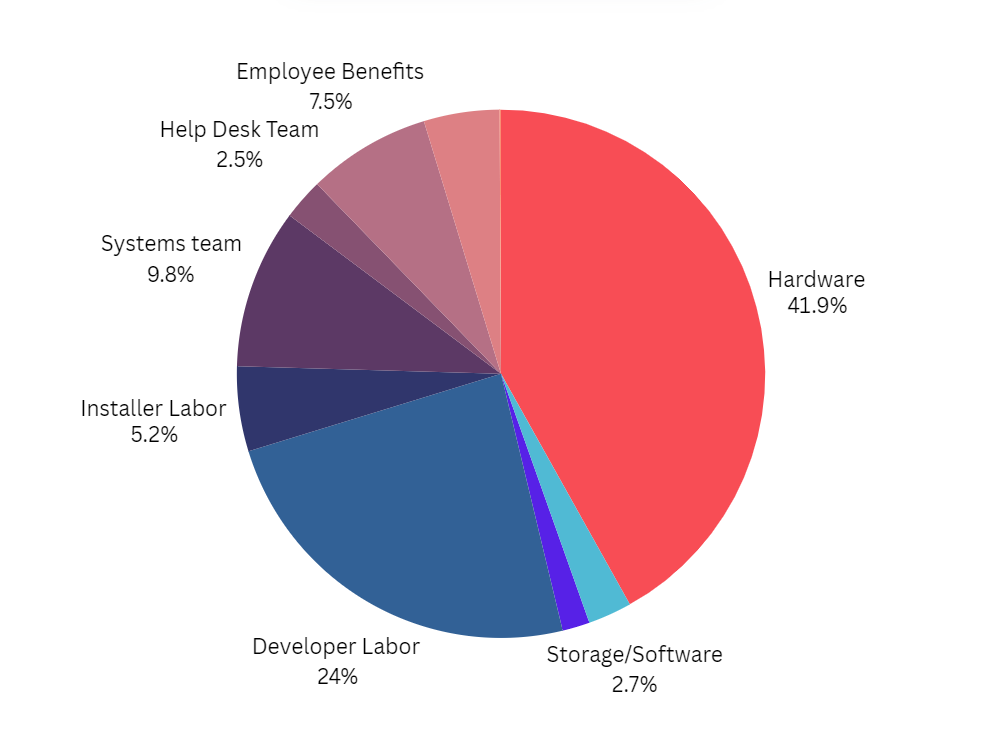
\includegraphics[width=\linewidth]{pi_chart.png}
    \caption{Costs broken down}
\end{figure}
<<<<<<< HEAD
\end{document}
=======
>>>>>>> refs/remotes/origin/main

\begin{thebibliography}{9}
    \bibitem{aws} Amazon Web Services (AWS). ``Amazon S3 Pricing.'' AWS, \url{https://aws.amazon.com/s3/pricing/}. Accessed 9 March 2025.
    \bibitem{reolink1} Reolink. ``Security Camera Systems.'' Reolink, \url{https://reolink.com/}. Accessed 9 March 2025.
    \bibitem{reolink2} Reolink. ``5MP IP Security Camera System.'' Reolink, \url{https://reolink.com/blog/5mp-ip-security-camera-system-for-outdoor-use/}. Accessed 9 March 2025.
    \bibitem{raspberrypi} Raspberry Pi Foundation. ``Raspberry Pi 5.'' Raspberry Pi, \url{https://www.raspberrypi.com/}. Accessed 9 March 2025.
    \bibitem{coral} Google Coral. ``Coral USB Accelerator.'' Coral, \url{https://coral.ai/products/accelerator/}. Accessed 9 March 2025.
    \bibitem{tplink} Amazon. ``TP-Link TL-SF1005P 4-Port PoE Switch.'' Amazon, \url{https://www.amazon.com/}. Accessed 9 March 2025.
    \bibitem{netgear} Amazon. ``NETGEAR GS308PP 8-Port PoE Switch.'' Amazon, \url{https://www.amazon.com/}. Accessed 9 March 2025.
    \bibitem{tplink2} Amazon. ``TP-Link TL-SG1016PE 16-Port PoE Switch.'' Amazon, \url{https://www.amazon.com/}. Accessed 9 March 2025.
    \bibitem{deptdirsal} Salary. I.T. Deptartment Director Salary. Salary. \url{https://www.salary.com/research/salary/benchmark/information-technology-director-salary/roanoke-va}
    \bibitem{hdspec} Ziprecruiter. Helpdesk Specialist Salary. Ziprecruiter. \url{https://www.ziprecruiter.com/Salaries/It-Support-Engineer-Salary--in-Virginia#:~:text=How%20much%20does%20an%20It,%2Fweek%20or%20%245%2C442%2Fmonth}
    \bibitem{nsspec} Ziprecruiter. Network Security Specialist Salary. Ziprecruiter. \url{https://www.ziprecruiter.com/Salaries/Network-Security-Engineer-Salary--in-Virginia#:~:text=As%20of%20Feb%2028%2C%202025,%2Fweek%20or%20%2410%2C323%2Fmonth}
    \bibitem{sysadmin} Ziprecruiter. System Administrator Salary. Ziprecruiter. \url{https://www.ziprecruiter.com/Salaries/Systems-Administrator-Salary--in-Virginia}
    \bibitem{sensoftdev} Ziprecruiter. Senior Software Developer Salary. Ziprecruiter. \url{https://www.salary.com/research/salary/alternate/senior-software-engineer-salary/va}
    \bibitem{jrsoftfdev} Ziprecruiter. Junior Software Developer Salary. Ziprecruiter. \url{https://www.ziprecruiter.com/Salaries/Junior-Software-Engineer-Salary--in-Virginia}
    \bibitem{basm} Ziprecruiter. Business Analyst Scrum Master  Salary. Ziprecruiter. \url{https://www.ziprecruiter.com/Jobs/Business-Analyst-Scrum-Master/--in-Virginia?lvk=DzIg93pBUD6xgHsdZitbwQ.--Njl8FSuQB}
    \bibitem{cengage} Seagate. (n.d.). Surveillance Storage Calculator | Seagate US. Seagate.com. \url{ https://www.seagate.com/video-storage-calculator/#}
\end{thebibliography}

\end{document}